\documentclass{article}
\usepackage[margin=1in]{geometry}
\usepackage{amsmath,amsthm,amssymb}
\usepackage{bbm,enumerate,mathtools}
\usepackage{tikz,pgfplots}
\usepackage{chessboard}
\usepackage[hidelinks]{hyperref}
\usepackage{multicol} % Problem 35

\newenvironment{question}{\begin{trivlist}\item[\textbf{Question.}]}{\end{trivlist}}
\newenvironment{note}{\begin{trivlist}\item[\textbf{Note.}]}{\end{trivlist}}
\newenvironment{references}{\begin{trivlist}\item[\textbf{References.}]}{\end{trivlist}}
\newenvironment{related}{\begin{trivlist}\item[\textbf{Related.}]\end{trivlist}\begin{enumerate}}{\end{enumerate}}


\begin{document}
\rating{4}{2}
It turns out that the rational numbers $\mathbb{Q}$ can be generated starting from $0$ by iterating the two maps $f(x) = x + 1$ and $g(x) = -1/x$. This is because $f$ and $g$ generate the modular group $\Gamma$, and $g \circ f \circ g \circ f \circ g = f^{-1}$ and $g = g^{-1}$.

We can use this fact to create the tree in OEIS sequence \href{https://oeis.org/A226247}{A226247}, which is shown below.
\begin{figure}[ht!]
  \centering
  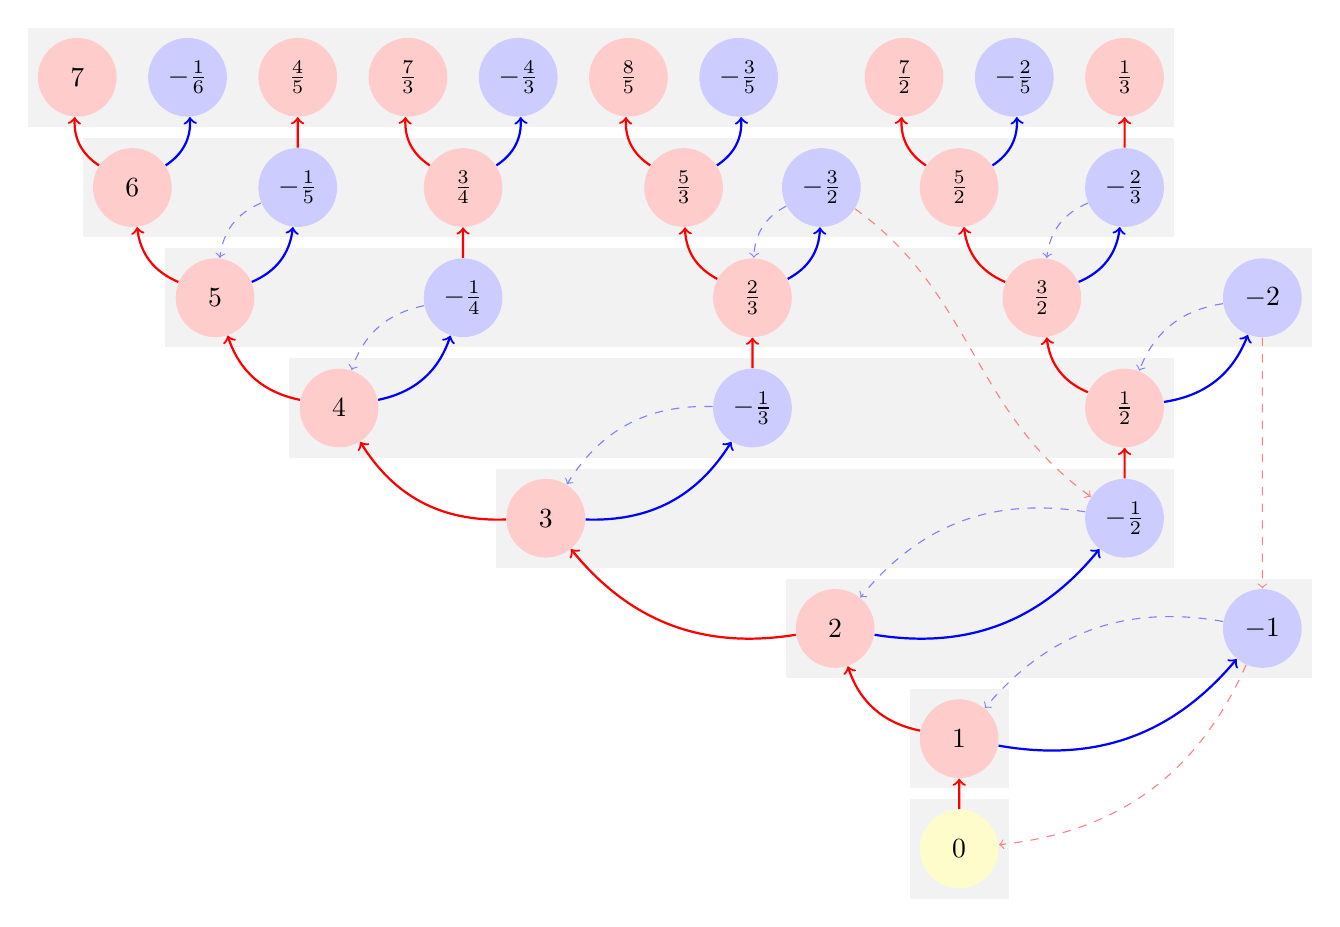
\begin{tikzpicture}[scale=1.4]
    \fill[black, opacity=0.05] (2.55,-0.45)  rectangle (3.45,0.45);
    \fill[black, opacity=0.05] (2.55,0.55)   rectangle (3.45,1.45);
    \fill[black, opacity=0.05] (1.425,1.55)  rectangle (6.2,2.45);
    \fill[black, opacity=0.05] (-1.2,2.55)   rectangle (4.95,3.45);
    \fill[black, opacity=0.05] (-3.075,3.55) rectangle (4.95,4.45);
    \fill[black, opacity=0.05] (-4.2,4.55)   rectangle (6.2,5.45);
    \fill[black, opacity=0.05] (-4.95,5.55)  rectangle (4.95,6.45);
    \fill[black, opacity=0.05] (-5.45,6.55)  rectangle (4.95,7.45);

    % Rank 0
    \node[circle, minimum size=1.0cm, fill=yellow!20!white] (00) at (3,0) {$0$};
    % \draw[dotted,fill opacity=0.05, fill=black] (2.55,-0.45) rectangle (3.45,0.45);
    % Rank 1
    \node[circle, minimum size=1.0cm, fill=red!20!white] (10) at (3,1) {$1$};
    % \draw[dotted,fill opacity=0.05, fill=black] (2.55,0.55) rectangle (3.45,1.45);
    % Rank 2
    \node[circle, minimum size=1.0cm, fill=blue!20!white] (20) at (5.75,2) {$-1$};
    \node[circle, minimum size=1.0cm, fill=red!20!white] (21) at (1.875,2) {$2$};
    % \draw[dotted,fill opacity=0.05, fill=black] (1.425,1.55) rectangle (6.2,2.45);
    % Rank 3
    \node[circle, minimum size=1.0cm, fill=blue!20!white] (30) at (4.5,3) {$-\frac12$};
    \node[circle, minimum size=1.0cm, fill=red!20!white] (31) at (-0.75,3) {$3$};
    % \draw[dotted,fill opacity=0.05, fill=black] (-1.2,2.55) rectangle (4.95,3.45);
    % Rank 4
    \node[circle, minimum size=1.0cm, fill=red!20!white] (40) at (4.5,4) {$\frac12$};
    \node[circle, minimum size=1.0cm, fill=blue!20!white] (41) at (1.125,4) {$-\frac13$};
    \node[circle, minimum size=1.0cm, fill=red!20!white] (42) at (-2.625,4) {$4$};
    % \draw[dotted,fill opacity=0.05, fill=black] (-3.075,3.55) rectangle (4.95,4.45);
    % Rank 5
    \node[circle, minimum size=1.0cm, fill=blue!20!white] (50) at (5.75,5) {$-2$};
    \node[circle, minimum size=1.0cm, fill=red!20!white] (51) at (3.75,5) {$\frac32$};
    \node[circle, minimum size=1.0cm, fill=red!20!white] (52) at (1.125,5) {$\frac23$};
    \node[circle, minimum size=1.0cm, fill=blue!20!white] (53) at (-1.5,5) {$-\frac14$};
    \node[circle, minimum size=1.0cm, fill=red!20!white] (54) at (-3.75,5) {$5$};
    % \draw[dotted,fill opacity=0.05, fill=black] (-4.2,4.55) rectangle (6.2,5.45);

    \node[circle, minimum size=1.0cm, fill=blue!20!white] (60) at (4.5,6) {$-\frac23$};
    \node[circle, minimum size=1.0cm, fill=red!20!white] (61) at (3,6) {$\frac52$};
    \node[circle, minimum size=1.0cm, fill=blue!20!white] (62) at (1.75,6) {$-\frac32$};
    \node[circle, minimum size=1.0cm, fill=red!20!white] (63) at (0.5,6) {$\frac53$};
    \node[circle, minimum size=1.0cm, fill=red!20!white] (64) at (-1.5,6) {$\frac34$};
    \node[circle, minimum size=1.0cm, fill=blue!20!white] (65) at (-3,6) {$-\frac15$};
    \node[circle, minimum size=1.0cm, fill=red!20!white] (66) at (-4.5,6) {$6$};
    % \draw[dotted,fill opacity=0.05, fill=black] (-4.95,5.55) rectangle (4.95,6.45);

    \node[circle, minimum size=1.0cm, fill=red!20!white] (70) at (4.5,7) {$\frac13$};
    \node[circle, minimum size=1.0cm, fill=blue!20!white] (71) at (3.5,7) {$-\frac25$};
    \node[circle, minimum size=1.0cm, fill=red!20!white] (72) at (2.5,7) {$\frac72$};
    \node[circle, minimum size=1.0cm, fill=blue!20!white] (73) at (1,7) {$-\frac35$};
    \node[circle, minimum size=1.0cm, fill=red!20!white] (74) at (0,7) {$\frac85$};
    \node[circle, minimum size=1.0cm, fill=blue!20!white] (75) at (-1,7) {$-\frac43$};
    \node[circle, minimum size=1.0cm, fill=red!20!white] (76) at (-2,7) {$\frac73$};
    \node[circle, minimum size=1.0cm, fill=red!20!white] (77) at (-3,7) {$\frac45$};
    \node[circle, minimum size=1.0cm, fill=blue!20!white] (78) at (-4,7) {$-\frac16$};
    \node[circle, minimum size=1.0cm, fill=red!20!white] (79) at (-5,7) {$7$};
    % \draw[dotted,fill opacity=0.05, fill=black] (-5.45,6.55) rectangle (4.95,7.45);

    % Edges
    \draw[thick, red, ->] (00) to (10);

    \draw[thick, red, bend left, ->] (10) to (21);
    \draw[thick, blue, bend right, ->] (10) to (20);
    \draw[dashed,blue!50!white, bend right, ->] (20) to (10);

    \draw[dashed,red!50!white, bend left, ->] (20) to (00);

    \draw[thick, red,bend left,->] (21) to (31);
    \draw[thick, blue,bend right,->] (21) to (30);
    \draw[dashed,blue!50!white, bend right, ->] (30) to (21);

    \draw[thick, red,->] (30) to (40);

    \draw[thick, red,bend left,->] (31) to (42);
    \draw[thick, blue,bend right,->] (31) to (41);
    \draw[dashed,blue!50!white, bend right, ->] (41) to (31);

    \draw[thick, red,bend left,->] (40) to (51);
    \draw[thick, blue,bend right,->] (40) to (50);
    \draw[dashed,blue!50!white, bend right, ->] (50) to (40);

    \draw[thick, red,->] (41) to (52);

    \draw[thick, red,bend left,->] (42) to (54);
    \draw[thick, blue,bend right,->] (42) to (53);
    \draw[dashed,blue!50!white, bend right, ->] (53) to (42);

    \draw[thick, red,bend left,->] (51) to (61);
    \draw[thick, blue,bend right,->] (51) to (60);
    \draw[dashed,blue!50!white, bend right, ->] (60) to (51);

    \draw[dashed,red!50!white, ->] (50) to (20);

    \draw[thick, red,bend left,->] (52) to (63);
    \draw[thick, blue,bend right,->] (52) to (62);
    \draw[dashed,blue!50!white, bend right, ->] (62) to (52);
    \draw[dashed,red!50!white, bend left, out=15, in=195, ->] (62) to (30);

    \draw[thick, red,->] (53) to (64);

    \draw[thick, red,bend left,->] (54) to (66);
    \draw[thick, blue,bend right,->] (54) to (65);
    \draw[dashed,blue!50!white, bend right, ->] (65) to (54);

    \draw[thick, red,->] (60) to (70);

    \draw[thick, blue,bend right,->] (61) to (71);
    % \draw[dashed,blue!50!white, bend right, ->] (71) to (61);
    \draw[thick, red,bend left,->] (61) to (72);

    \draw[thick, blue,bend right,->] (63) to (73);
    % \draw[dashed,blue!50!white, bend right, ->] (73) to (62);
    \draw[thick, red,bend left,->] (63) to (74);

    \draw[thick, blue,bend right,->] (64) to (75);
    % \draw[dashed,blue!50!white, bend right, ->] (73) to (62);
    \draw[thick, red,bend left,->] (64) to (76);

    \draw[thick, red,->] (65) to (77);

    \draw[thick, blue,bend right,->] (66) to (78);
    % \draw[dashed,blue!50!white, bend right, ->] (78) to (66);
    \draw[thick, red,bend left,->] (66) to (79);
  \end{tikzpicture}

  \caption{
    Caption.
  }
\end{figure}

\begin{question}
  Let $a(n)$ be the number of elements in the $n$-th rank. Does $a(n) = a(n-1) + a(n-3)$ for all $n \geq 4$?
\end{question}

\begin{related}
  \item In the figure above, the vertices numbers whose last application is $g(x) = -1/x$ are colored blue. Is a vertex blue if and only if its value is negative?
  \item Is there a way to characterize all rank $n$ rational numbers?
\end{related}

\begin{note}
  Math Stack Exchange, ``\href{https://math.stackexchange.com/q/5057812/121988}{Enumerating all fractions by $x \mapsto x + 1$ and $x \mapsto -1/x$}.''
\end{note}
\end{document}
